\section{Benchmarking the Implementation Schemes}
\label{bench}

In this section we want to evaluate Scala library in terms of the impact that the cooperative scheduling feature has on performance. We will use a benchmark that involves heavy cooperative scheduling to compare the data-oriented approach to the process-oriented approach that ABS when translated to Java. Furthermore we will use a benchmark tailored towards CPU-intensive to evaluate the potential of this Scala library to support ABS as a software-development language. We will compare our solution with both the Erlang backend of ABS which benefits from lightweight threads as well as the Akka Actor library for Scala.

\subsection{Cooperative Scheduling Benchmark}
The main problem that we encountered when implementing cooperative scheduling was saving the context of an execution and resuming from that context. To do this in Java using threads and context switches heavily limits the application to the number of native threads that can be created.  To measure the improvement provided by our Scala library features using the simple example that is illustrated in Listing ~\ref{absex} that is translated into Scala as Listing~\ref{scalaex}.

%In the
%example we have one actor containing an which receives a large
%number of messages stored in its queue. This message recursively calls
%a function that creates a stack frame after which a message is
%sent to a different Actor to run in parallel a function that computes a large number of trigonometric operations . The object is then suspended to await the
%result of this function, resulting in the requirement to save the stack frame in order to allow the next message from the queue to run
%on the actor. We varied the total number
%of messages in the object's queue to compare performance between a trivial thread based approach and our optimized solution in the Java backend for ABS. 

%\begin{figure}
%	\label{sf}
%	\centering
%	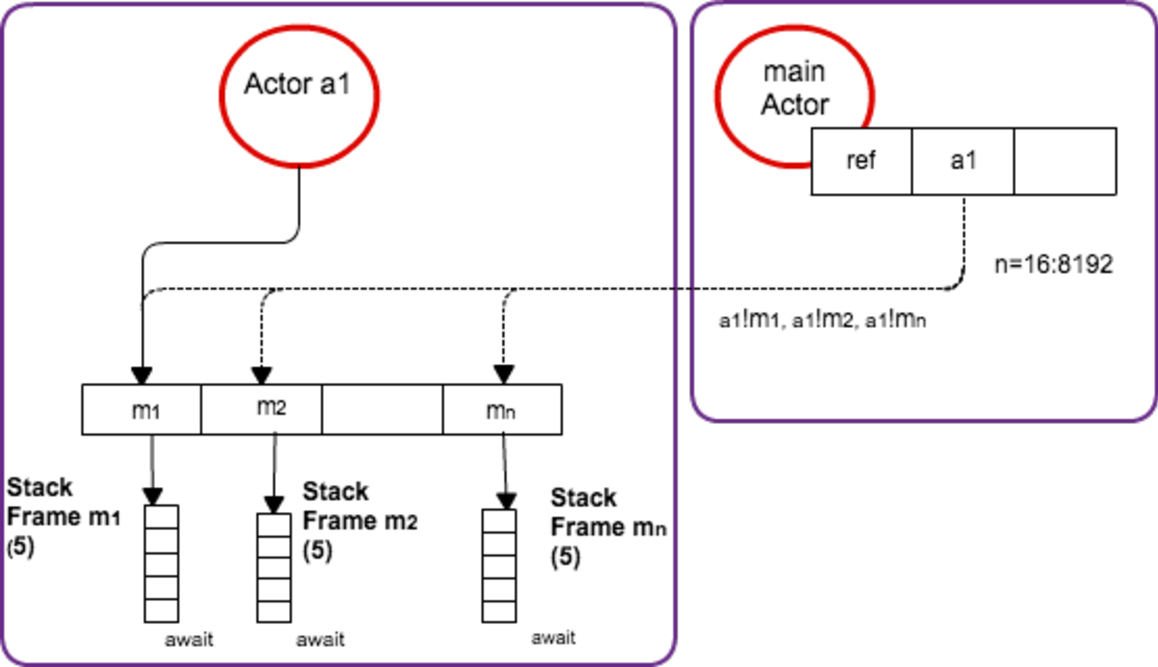
\includegraphics[scale=0.6]{scenario}
%	\caption{Cooperative Scheduling Benchmark Scenario}
%\end{figure}
\begin{lstlisting}[caption= Benchmark Example, label=scalaex]
trait Ainterface extends Actor with Ordered[Actor] {
	def recursive_m( i : Int,  id : Int): Int;
}

class A() extends LocalActor with Ainterface {

	var result : Int =  0;
	
	def recursive_m( i : Int,  id : Int): Int= {
		if ((i > 0)) {
			var msg : Callable[Int] = () => this.recursive_m((i - 1), id);
			var future_k : ABSFutureTask[Int]  
						= this.sendSync ((future_k_par: ABSFutureTask[Int])=>
								this.Arecursive_mAwait0(i, id, future_k_par), msg);
			var k : Int   = future_k.get();
		}
		else {
			var msg : Callable[Int] = () => this.compute();
			var f : ABSFutureTask[Int] = this.send (msg);
			await(()=>this.Arecursive_mAwait1(f, i, id), Guard.convert(f));
		}
		return 1;
	}
	
	def compute(): Int= {
		result = (result + 1);
		return result;
	}
	
	def Arecursive_mAwait0( i : Int,  id : Int,  future_k : ABSFutureTask[Int]): Int= {
		var k : Int = future_k.get();
		return 1;
	}
	
	def Arecursive_mAwait1( f : ABSFutureTask[Int],  i : Int,  id : Int): Int= {
		return 1;
	}
}

object Main extends LocalActor {

	def main( args : Array[String]): Unit= {
		var i : Int =  0;
		var master : Ainterface =  new A();
		var futures : List[ABSFutureTask[Int]] =  Nil();
		
		while ((i < 2000)) {
			var msg : Callable[Int] = () => master.recursive_m(5, i);
			var f : ABSFutureTask[Int] = master.send (msg);
			futures = Cons(f, futures);
			i = (i + 1);
		}
		
		while ((!Objects.equals(futures, Nil[ABSFutureTask[Int]]()))) {
			var f1 : ABSFutureTask[Int] =  head(futures);
			futures = tail(futures);
			var r : Int = f1.get();
}	}	}
\end{lstlisting}

\par The model creates an Actor of type "A" and sends a large number of messages to it to execute a method \lstinline|recursive_m(5,i|. This method creates a call chain of size 5 before sending an asynchronous message to itself to execute a basic method \lstinline|compute()| and awaits on its result. Although simple, this example allows us to benchmark the pure overhead that arises from having a runtime system with cooperative scheduling support, both in a data-oriented approach and a process-oriented approach. The results are shown in Figure~\ref{jj}. The performance figures presented are for one actor that is running 500-2500 method invocations. It is important to observe that each invocation generates 2 messages in the actor’s queue, so as the number of calls increases the number of messages doubles. The figures show that the trade-off for storing continuations into memory instead of saving them in native threads removes limitations on the application and significantly reduces overhead. 

\begin{figure}
	\centering
	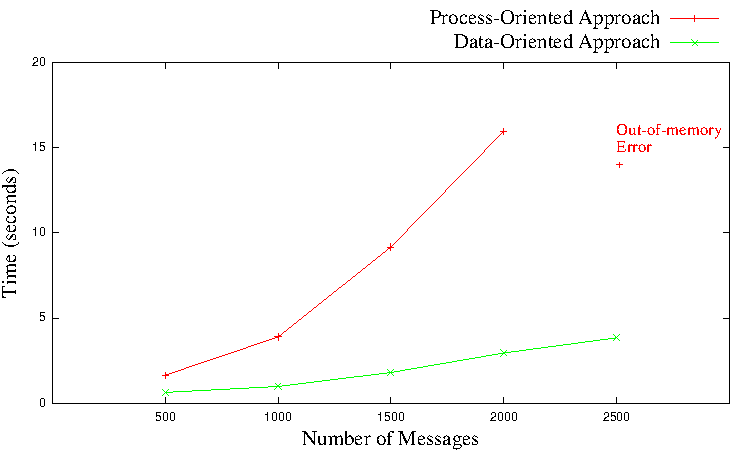
\includegraphics[scale=.68]{jaj8.pdf}
	\caption{Performance figures for pure Cooperative Scheduling}
	\label{jj}
\end{figure}

%loc
\subsection{NQueens Benchmark}
\par While our solution is catered towards a widely-used software development language, we would like to also compare with other languages that implement ABS language concepts efficiently using threads and without these limitations. In Section~\ref{run} we listed several optimizations that were inferred from our implementation solution. What we want to do is compare this optimized solution to an ABS backend implemented in Erlang that uses the same process-oriented approach but does not suffer from any limitation of native threads. We want to observe if our data-oriented approach can be comparable to Erlang's lightweight threads. For this comparison, we use the Savina benchmark for programming with actors~\cite{savina}.  We chose the problem of arranging $N$ queens on a $NxN$ chessboard as it provides a master-slave model that relies heavily on the cooperative scheduling properties of the master model.  The benchmark divides the task of finding all the valid solutions to the $N$ queens problem to a fixed number of workers that at each step have to find an intermediary solution of placing a queen $K$ on the board before relaying the message back to the master which then assigns the next job of placing queen $K+1$ to another worker. As the search space becomes smaller, w impose a threshold where the worker has to find the complete solution up to $N$ queens before sending a message back to the master. 
\par We ran the benchmark with a board size varying from 6 to 12 with a fixed number of 4 workers on a core i5 machine which supports hyper-threading. The results are shown in Figure~\ref{jj}. It is important to observe that as the board size increases, the number of solutions grows from 40 to 2680. The result in Figure~\ref{ej} show that our approach is better once the board size reaches 12 and the number of solutions to be found is 14200. This result also strengthens ABS purpose to provide a programming language for real applications.

\begin{figure}
	\centering
	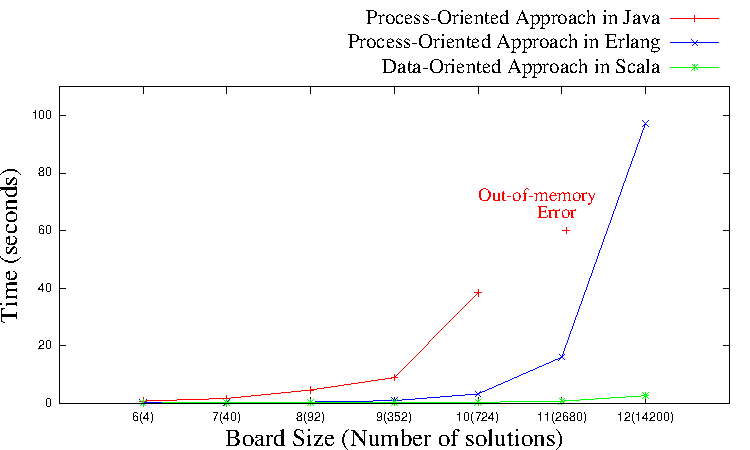
\includegraphics[scale=.7]{erlj8.pdf}
	\caption{Performance figures for the NQueens problem in 3 ABS backends}
	\label{ej}
\end{figure}

\par Furthermore, we would like to observe the performance impact that support for cooperative scheduling adds to an application. This feature is a powerful programming concept, but we would like to see the cost of developing a benchmark in comparison to an existing actor implementation like the Akka Actor library. It is first important to observe that the ABS model for this benchmark is 154 lines of code, while the benchmark written directly in Scala using the Akka library is 351 lines of code. We compared the implementation offered by the Savina benchmark with our own for a board size from 10  to 15 on the same machine as before. The results in Figure\ref{aj} show that the cooperative scheduling feature does not have any added overhead compared to the Akka Actor library while offering a seamless programming experience.

\begin{figure}
\centering
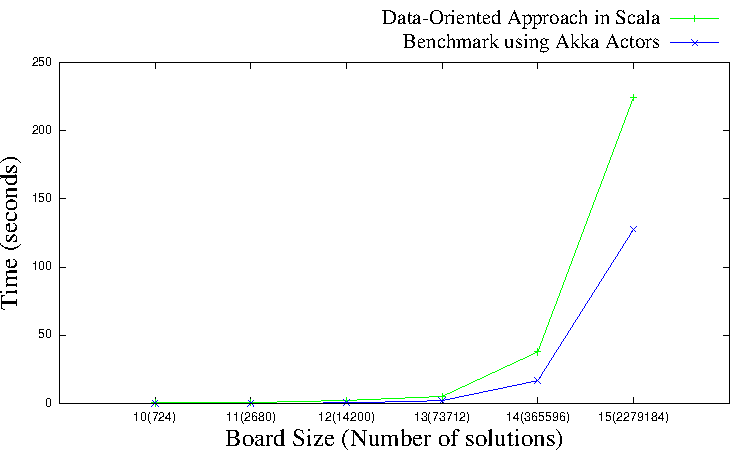
\includegraphics[scale=.7]{akka8.pdf}
\caption{Performance figures for the NQueens problem implementations in Akka and Scala Library}
\label{aj}
\end{figure}

%To measure the improvement provided by Java 8 features, we use the Savina benchmark for programming with actors~\cite{savina}.  We chose the problem of arranging $N$ queens on a $NxN$ chessboard as it provides a master-slave model that relies heavily on the cooperative scheduling properties of the master model.  The benchmark divides the task of finding all the valid solutions to the $N$ queens problem to a fixed number of workers that at each step have to find an intermediary solution of placing a queen $K$ on the board before relaying the message back to the master which then assigns the next job of placing queen $K+1$ to another worker. As the search space becomes smaller, w impose a threshold where the worker has to find the complete solution up to $N$ queens before sending a message back to the master.
% \par We benchmarked the performance of both a data-oriented approach and a process-oriented approach with 


%\par These results do show the drawback of native Java threads. However, while our solution is catered towards a widely-used software development language, it doesn't mean that there aren't other languages that are more suited to implement ABS language concepts efficiently using threads and without these limitations. In Section~\ref{optimizations} we listed several optimizations that were inferred from our implementation solution. What we want to do is compare this optimized solution to an ABS backend implemented in Erlang that uses the same process-oriented approach but does not suffer from any limitation of native threads. We want to observe if our data-oriented approach can be comparable to Erlang's lightweight threads. 





